\subsection{Movement Testing}
\label{subsec:movementtesting}

\begin{figure} [ht]
  \centering
  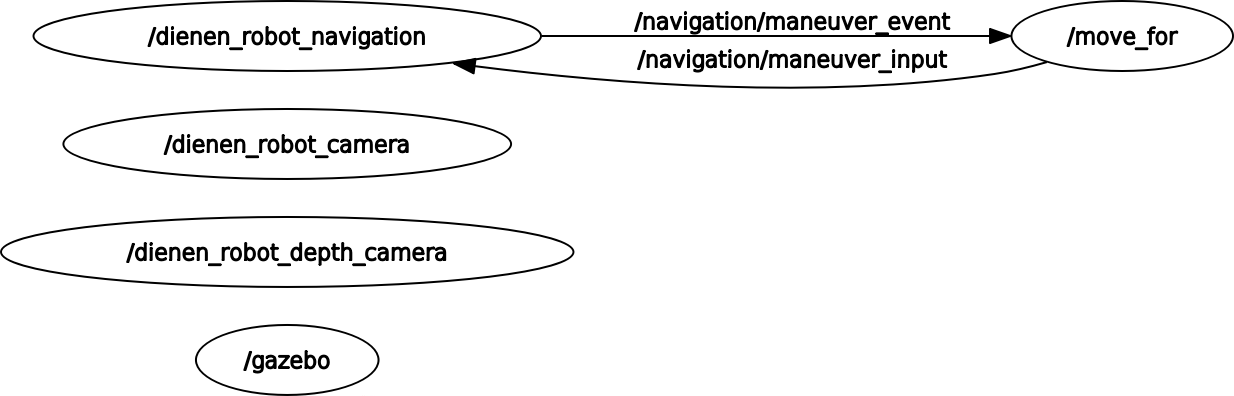
\includegraphics[width=0.45\textwidth]{images/rosgraph-simulation-movement-test.png}
  \caption{Node scheme of the movement testing in the simulation.}
  \label{fig:rosgraphsimulationmovementtest}
\end{figure}

\begin{figure} [ht]
  \centering
  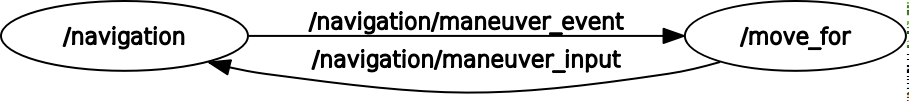
\includegraphics[width=0.45\textwidth]{images/rosgraph-real-robot-movement-test.png}
  \caption{Node scheme of the movement testing on the real robot.}
  \label{fig:rosgraphrealrobotmovementtest}
\end{figure}

Movement testing is done by running the \lstinline{move_for} node as a behavior node that will instruct the robot to move at a certain speed for a certain period of time.
As shown in Figure \ref{fig:rosgraphsimulationmovementtest},
  in the simulation,
  the \lstinline{move_for} node will be connected to the \lstinline{dienen_robot_navigation} node to control the speed of the robot using the \lstinline{/navigation/maneuver_input} topic.
As for testing in the real world, as shown in Figure \ref{fig:rosgraphrealrobotmovementtest},
  the role of the \lstinline{dienen_robot_navigation} node which manages the navigation on the virtual robot will be replaced by the \lstinline{navigation} node which manages the navigation on the real robot.

\begin{table}
  \caption{Linear movement test results in the simulation.}
  \label{tab:simulationlineartestresults}
  \centering
  \begin{tabular}{cc|cc|cc}
    \toprule
    \multicolumn{2}{c|}{Linear Speed} &
    \multicolumn{2}{|c|}{Simulation Position} &
    \multicolumn{2}{|c}{Odometry Position} \\
    \midrule
    x (m/min) & y (m/min) & x (m) & y (m) & x(m)  & y(m) \\
    \midrule
    40        & 0         & 5.2   & 0.0   & 5.2   & 0.0 \\
    60        & 0         & 7.9   & 0.0   & 7.9   & 0.0 \\
    -40       & 0         & -5.2  & 0.0   & -5.2  & 0.0 \\
    0         & 40        & 0.0   & 5.4   & 0.0   & 5.4 \\
    0         & -40       & 0.0   & -5.3  & 0.0   & -5.3 \\
    40        & 20        & 5.0   & 3.0   & 5.0   & 3.0 \\
    -20       & 40        & -2.9  & 5.5   & -2.9  & 5.5 \\
    \bottomrule
  \end{tabular}
\end{table}

\begin{table}
  \caption{Angular movement test results in the simulation.}
  \label{tab:simulationangulartestresults}
  \centering
  \begin{tabular}{c|c|c}
    \toprule
    Angular Speed   & Simulation Orientation & Odometry Orientation \\
    \midrule
    z (rad/min) & z (deg)               & z (deg) \\
    \midrule
    40          & 39.0                  & 39.0 \\
    120         & 118.7                 & 118.7 \\
    -40         & -39.2                 & -39.2 \\
    -120        & -117.1                & -117.1 \\
    \bottomrule
  \end{tabular}
\end{table}

The movement test is divided into two parts,
  linear movement testing and angular movement testing,
  each is tested for 10 seconds on a virtual robot in a simulation environment and on a real robot in the real world.
As shown in Table \ref{tab:simulationlineartestresults} and Table \ref{tab:simulationangulartestresults},
  the position and orientation of the odometry received by the robot has the same value as the position and orientation of the robot model in the simulation.
This happens because the odometry value sent by the \lstinline{dienen_robot_navigation} node is the same value as the robot model transformation in the simulation.

\begin{table}
  \caption{Linear movement test results on the real robot.}
  \label{tab:realrobotlineartestresults}
  \centering
  \begin{tabular}{cc|cc|cc}
    \toprule
    \multicolumn{2}{c|}{Linear Speed} &
    \multicolumn{2}{|c|}{Real World Position} &
    \multicolumn{2}{|c}{Odometry Position} \\
    \midrule
    x (m/min) & y (m/min) & x (m) & y (m) & x(m)  & y(m) \\
    \midrule
    40        & 0         & 5.1   & -0.1  & 5.2   & 0.1 \\
    60        & 0         & 8.1   & 0.1   & 7.9   & 0.0 \\
    -40       & 0         & -5.3  & 0.1   & -5.2  & 0.1 \\
    0         & 40        & 0.0   & 5.4   & 0.1   & 5.2 \\
    0         & -40       & 0.2   & -5.1  & -0.1  & -5.5 \\
    40        & 20        & 5.2   & 3.1   & 5.3   & 3.1 \\
    -20       & 40        & -3.1  & 5.3   & -2.9  & 5.3 \\
    \bottomrule
  \end{tabular}
\end{table}

\begin{table}
  \caption{Angular movement test results on the real robot.}
  \label{tab:realrobotangulartestresults}
  \centering
  \begin{tabular}{c|c|c}
    \toprule
    Angular Speed   & Real World Orientation  & Odometry Orientation \\
    \midrule
    z (rad/min) & z (deg)                   & z (deg) \\
    \midrule
    40          & 41.0                      & 39.6 \\
    120         & 120.0                     & 119.3 \\
    -40         & -40.0                     & -39.6 \\
    -120        & -119.0                    & -116.2 \\
    \bottomrule
  \end{tabular}
\end{table}

In contrast to the movement testing in the simulation environment,
  movement testing in the real world have different results between direct measurements and the odometry values received by the robot.
As shown in Table \ref{tab:realrobotlineartestresults} and Table \ref{tab:realrobotangulartestresults},
  there is a difference between the two value due to inaccuracies in the sensors used to obtain position and orientation values.
However, despite the differences in the level of accuracy, by using the same node behavior,
  the robot is capable of carrying out appropriate movement commands when tested in the simulation and the real world.
